\documentclass[]{article}
\usepackage[utf8]{inputenc}
\usepackage[a4paper]{geometry}  \geometry{hmargin=1.5cm,vmargin=1.5 cm}
\usepackage{xcolor}
\usepackage{amsmath}
\usepackage{amssymb}
\usepackage{amsfonts}
\usepackage{booktabs}
\usepackage{amsthm}
\usepackage{array}
\usepackage{epsfig}
\usepackage{caption}
\usepackage{empheq}
\usepackage{multicol}
\captionsetup{position=below}
\setlength{\parindent}{0pt}
\usepackage{graphicx}
\usepackage{color}
\usepackage{fancybox}
\usepackage{listings}
\usepackage{hyperref}
\usepackage{euscript}
\usepackage{float}
\usepackage{cite}


\theoremstyle{plain}
\newtheorem{theorem}{Théorème}
\newtheorem{lemma}[theorem]{Lemme}
\newtheorem{corollary}[theorem]{Corollaire}
\newtheorem{proposition}[theorem]{Proposition}
\newtheorem{example}[theorem]{Exemple}

\theoremstyle{remark}
\newtheorem{remark}{Remarque}

\begin{document}

\begin{center} 
	\huge Figures annex
\end{center}

\section*{RANS}

\begin{figure}[h]
	\begin{center}
	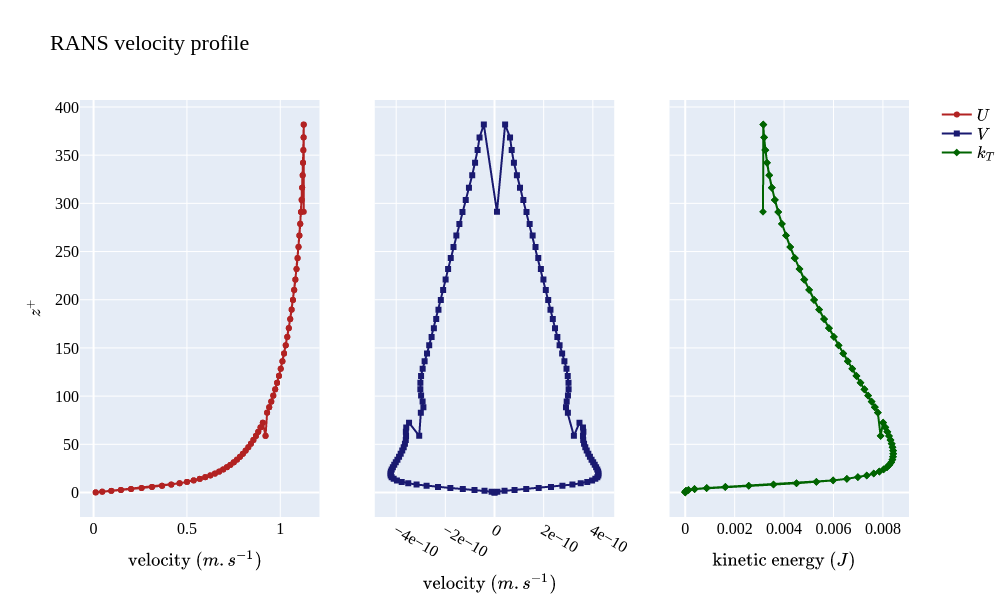
\includegraphics[width=\textwidth]{../output/RANS/profiles.png}
	\caption{The two velocity profiles of streamwise velocity (left) and spanwise velocity (middle) and the kinetic energy profile (right). They are ploted in function of $z^+$. It seems that we have two outlier points. The last point and one between $z^+=50$ and $z^+=100$}
	\end{center}
\end{figure}



\section*{Velocity analyses}
\newpage

\begin{figure}[h!]
	\begin{center}
	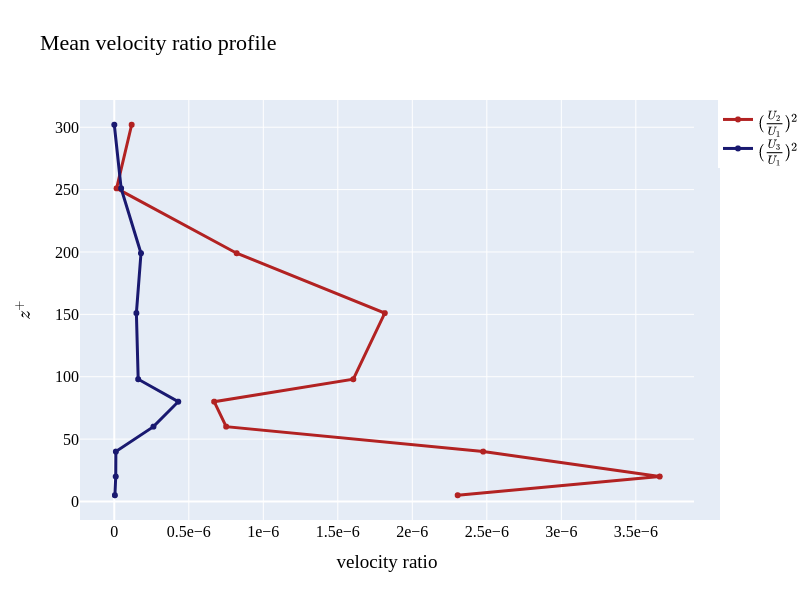
\includegraphics[width=\textwidth]{../output/velocity_profile.png}
	\caption{Square ratio of the spanwise on streamwise velocity (red) and the wall-normal on streamwise velocity (blue). They have been calculated taking the 10 streamwise plans. The streamwise velocity appears to be very dominant on both the spanwise and the wall-normal velocity.}
	\end{center}
\end{figure}

\section*{Frozen turbulence}
We want to verify the frozen turbulence hypotethis which state that $\phi_{ij}^{[1]}(k_1,x_2,x_3)=U_c\psi_{ij}(U_ck_1,x_2,x_3)$ with $\omega=U_ck_1$. $U_c$ is the mean streamwise velocity, $\phi_{ij}^{[1]}$ is the spatial spectra in the streamwise direction and $\psi_{ij}$ is the time spectra.
\subsection*{Power spectras}

\begin{figure}[h!]
	\begin{center}
		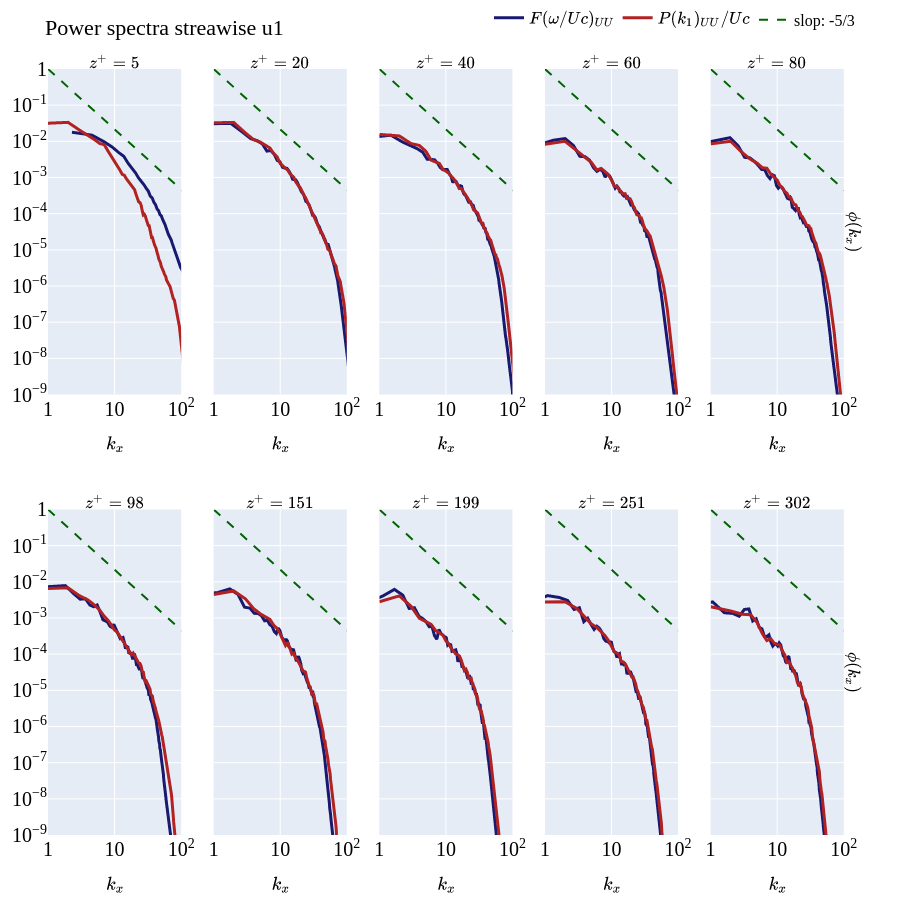
\includegraphics[width=0.9\textwidth]{../output/split_time/frozen_turbulence/power_spectra/u1_all.png}
	\end{center}
\end{figure}

\begin{figure}[h!]
	\begin{center}
		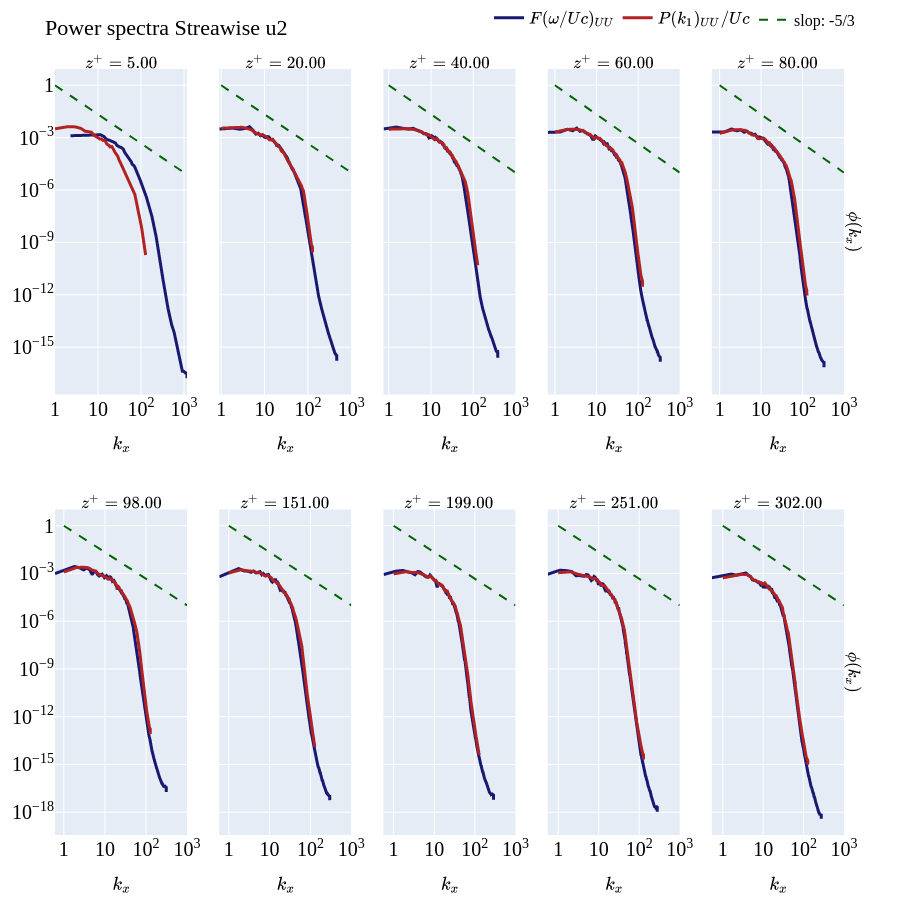
\includegraphics[width=0.9\textwidth]{../output/split_time/frozen_turbulence/power_spectra/u2_all.png}
	\end{center}
\end{figure}

\begin{figure}[h!]
	\begin{center}
		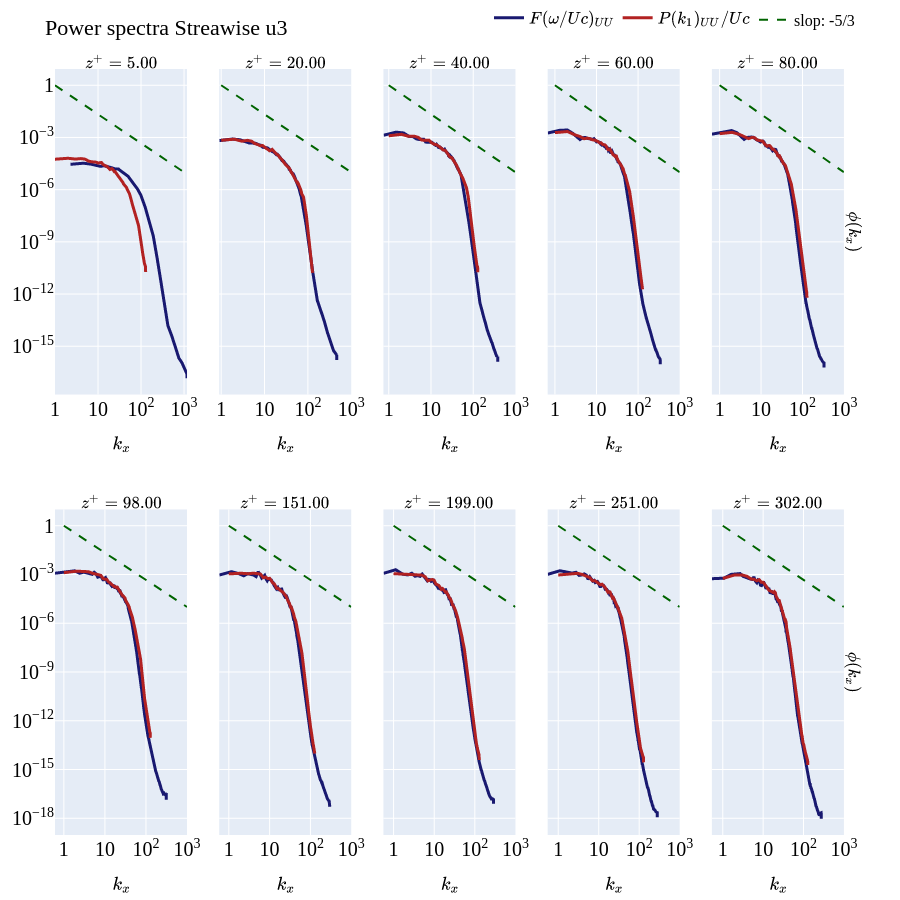
\includegraphics[width=0.9\textwidth]{../output/split_time/frozen_turbulence/power_spectra/u3_all.png}
		\caption{Power spectra in space (red) and time (blue) for the streamwise velocity (top), spanwise velocity (middle) and wall-normal velocity (bottom) at 10 different heights. The Uc took is the mean velocity along the streamwise axis}
	\end{center}
\end{figure}

\section*{Spatial correlations}


\begin{figure}[h!]
	\begin{center}
		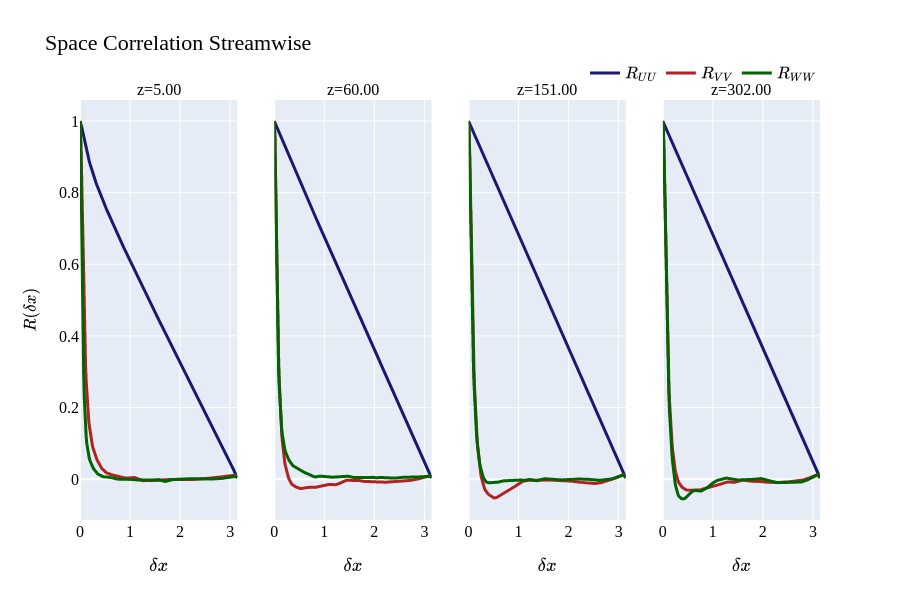
\includegraphics[width=0.9\textwidth]{../output/split_time/space_correlation/streamwise.png}
	\end{center}
\end{figure}

\begin{figure}[h!]
	\begin{center}
		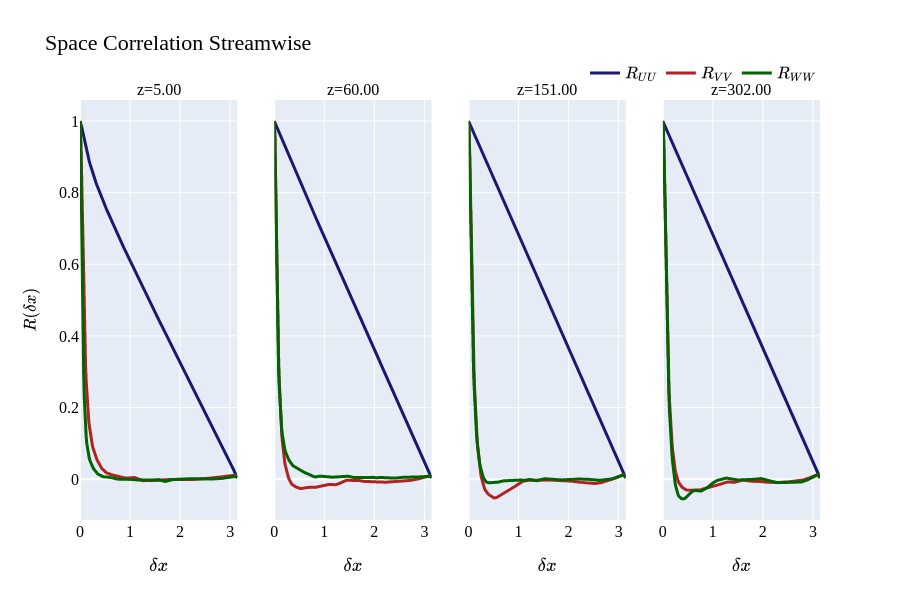
\includegraphics[width=0.9\textwidth]{../output/split_time/space_correlation/streamwise.png}
		\caption{Spatial correllation in a streamwise plan (top figure) andd in a spanwise plan (bottom figure). $U$ is the streamwise, $V$ the spanwise and $W$ the wall-normal velocities}
	\end{center}
\end{figure}


\section*{Gamma coefficient determination}

\begin{figure}[h!]
	\begin{center}
		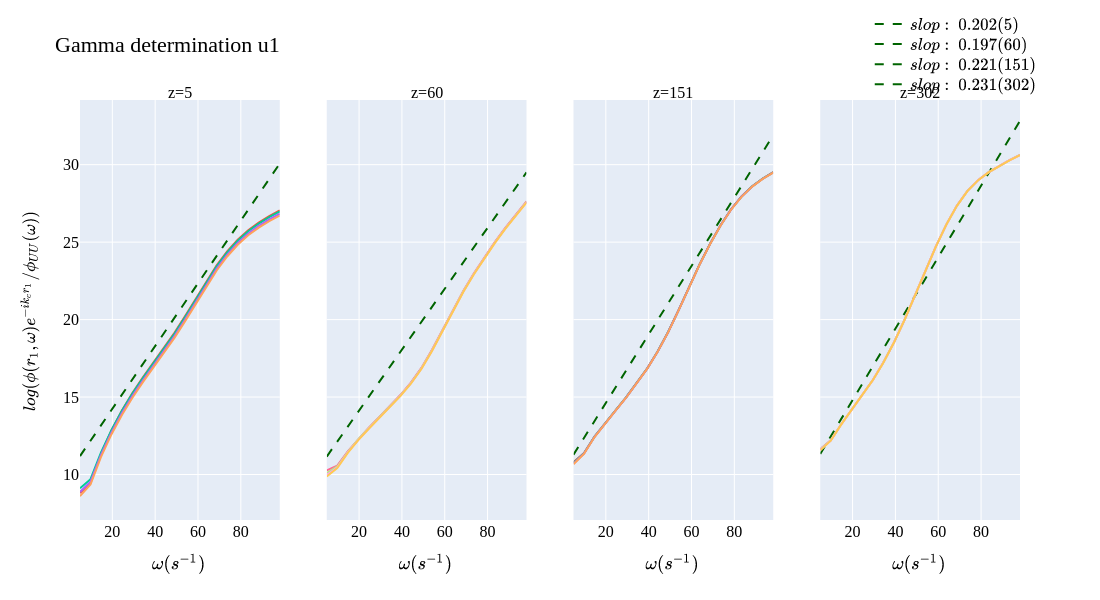
\includegraphics[width=0.9\textwidth]{../output/split_time/gamma/gamma_u1.png}
	\end{center}
\end{figure}

\begin{figure}[h!]
	\begin{center}
		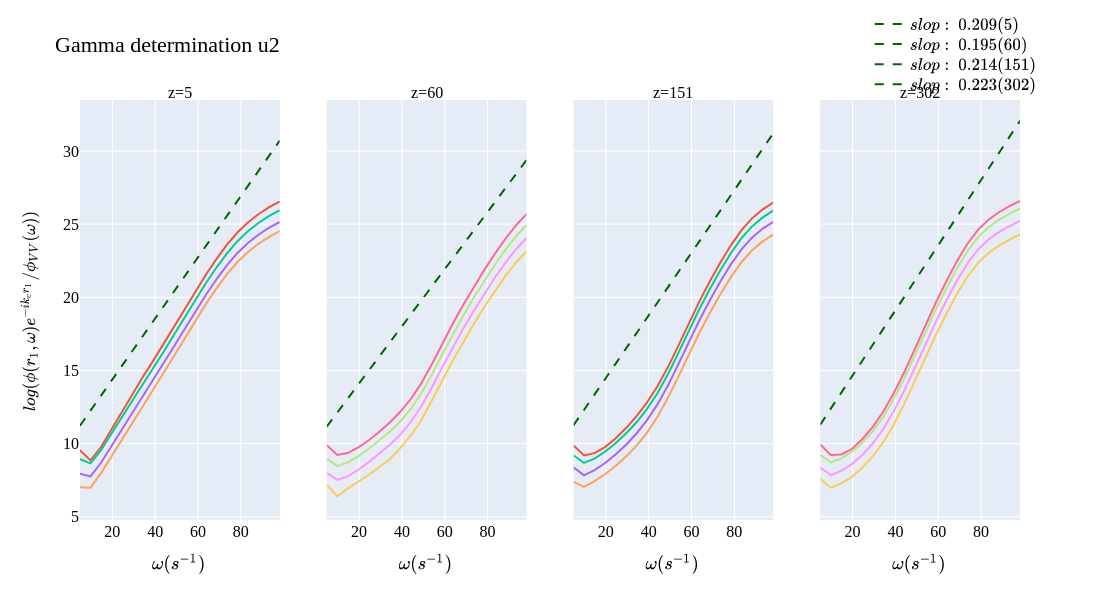
\includegraphics[width=0.9\textwidth]{../output/split_time/gamma/gamma_u2.png}
	\end{center}
\end{figure}

\begin{figure}[h!]
	\begin{center}
		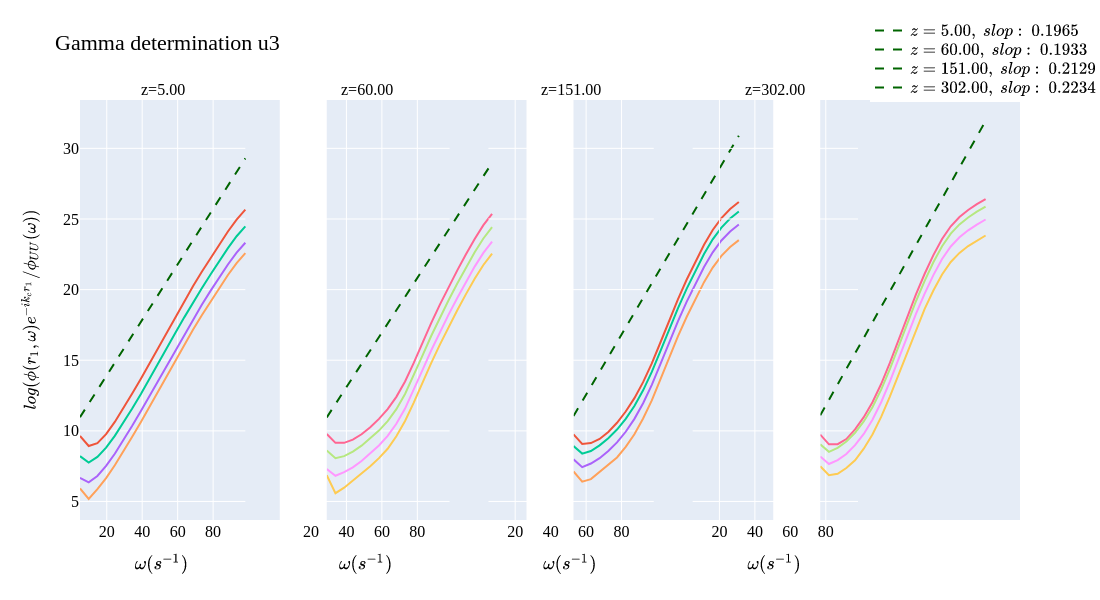
\includegraphics[width=0.9\textwidth]{../output/split_time/gamma/gamma_u3.png}
		\caption{Determination of $\gamma$ coefficient as $e^{-\gamma k_c r_1} = \frac{\phi(r_1,\omega)}{\phi_{ii}(\omega)}e^{-ik_cr_1}$. All these spectra are computed with streamwise plan with streamwise velocity (top figure), spanwise velocity (middle figure) and wall-normal velocity (bottom figure)}
	\end{center}
\end{figure}
	
	
\end{document}